\section{Aufgabe 15}
\textit{Implementieren sie als einfaches Bildverschlüsselungsverfahren eine Permutation der
Zeilen eines Bildes. Dazu soll als Parameter (z.B. 1, 2, 4, ...) eine Anzahl von
horizontalen Bildblöcken definiert werden können, innerhalb derer jeweils die Permutationen angewendet werden (also Permutationen auf das ganze Bild für 1, Permutationen innhalb der oberen und unteren Bildhälfte für 2, u.s.w.). Versuchen
sie anschliessend, unter Ausnutzung der Tatsache dass ähnliche Bildzeilen meist
nebeneinander liegen, eine Ciphertext only Attacke gegen das verschlüsselte Bild
(für verschiedene Parameterwerte und Bilder).}\vspace*{1em}\newline
Die Implementierung der Ver- und Entschlüsselung wurde vollständig in der Programmiersprache
\textbf{Rust} geschrieben. Zur Bildmanipulation wird das \href{https://docs.rs/image/latest/image/}{image} Crate verwendet. 
\subsection{Verschlüsselungsverfahren}
Um ein Bild zu verschlüsseln, wird es aus dem Speicher geladen und durch \verb|permutation_cipher| mit der
gewünschten Blockanzahl verschlüsselt. Für
dieses Experiment werden $1,2,4,8,16,32$ Blöcke mit unterschiedlichen Bildern getestet. 
\begin{verbatim}
let original = image::open(&path).expect("Failed to open image");

for blocks in [1, 2, 4, 8, 16, 32] {
    let cipher_image = permutation_cipher(&original, blocks);
    cipher_image
        .save(format!("./img/out/{:02}_{}", blocks, filename))
        .expect("Failed to save image");
}
\end{verbatim}
Normalerweiße würde man das Verschlüsselungsverfahren deterministisch anhand eines
Schlüssel durchführen. Für den Zweck dieses Experiments soll allerdings 
kein Schlüssel ermittelt werden, also können die Zeilen innerhalb eines Blocks
einfach gemischt werden. Zwei Zeilen eines Blocks werden zufällig ausgewählt und
getauscht. Dieser Vorgang wird dann $1000$ Mal wiederholt, 
um einen gut gemischten Block zu erhalten.
\begin{verbatim}
fn permutation_cipher(original: &image::DynamicImage, blocks: u32) 
    let mut img = original.to_rgba8();
    let rows_per_block = img.height() / blocks;

    for block in 0..blocks {
        for _ in 0..1000 {
            let row1 = rng().random_range(0..rows_per_block) + 
                block * rows_per_block;
            let row2 = rng().random_range(0..rows_per_block) + 
                block * rows_per_block;

            swap_rows(&mut img, row1, row2);
        }
    }

    image::DynamicImage::ImageRgba8(img)
}
\end{verbatim}
\begin{figure}[h]
    \centering
    \begin{subfigure}[b]{0.3\textwidth}
        \centering
        
\includegraphics[width=\textwidth]{./img/tloztotk.png}
        \caption{Original}
    \end{subfigure}
    \hfill
    \begin{subfigure}[b]{0.3\textwidth}
        \centering
        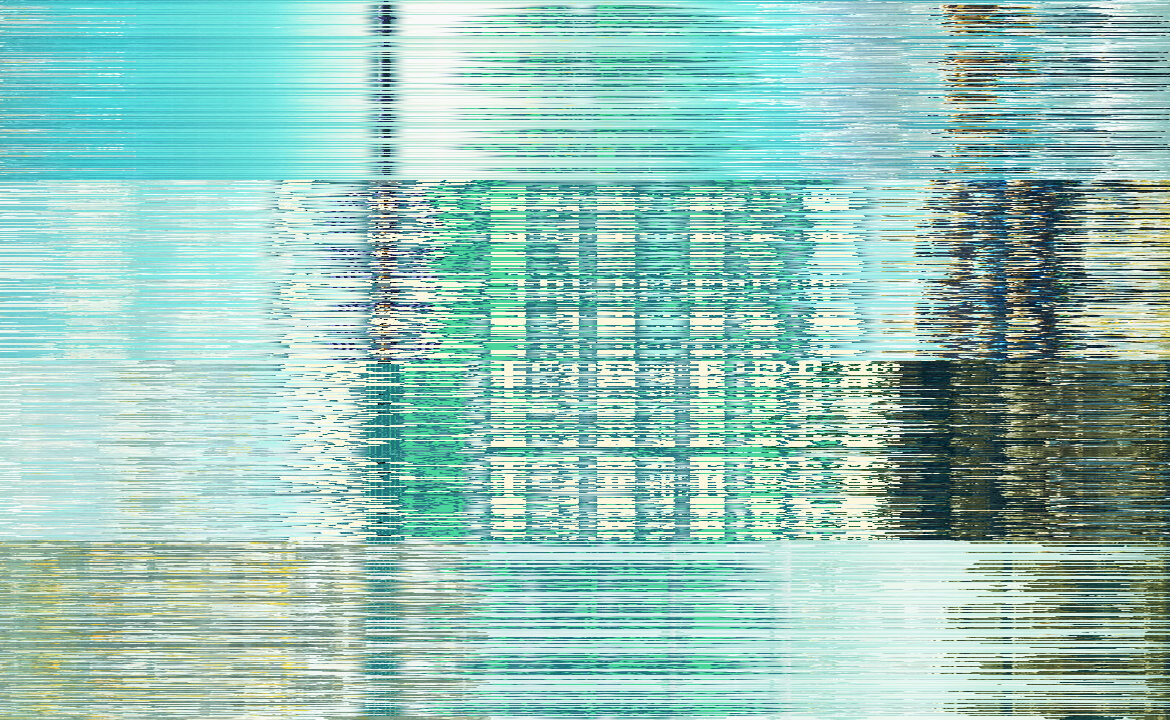
\includegraphics[width=\textwidth]{./img/cipher/04_tloztotk.png}
        \caption{4 Blöcke}
    \end{subfigure}
    \hfill
    \begin{subfigure}[b]{0.3\textwidth}
        \centering
        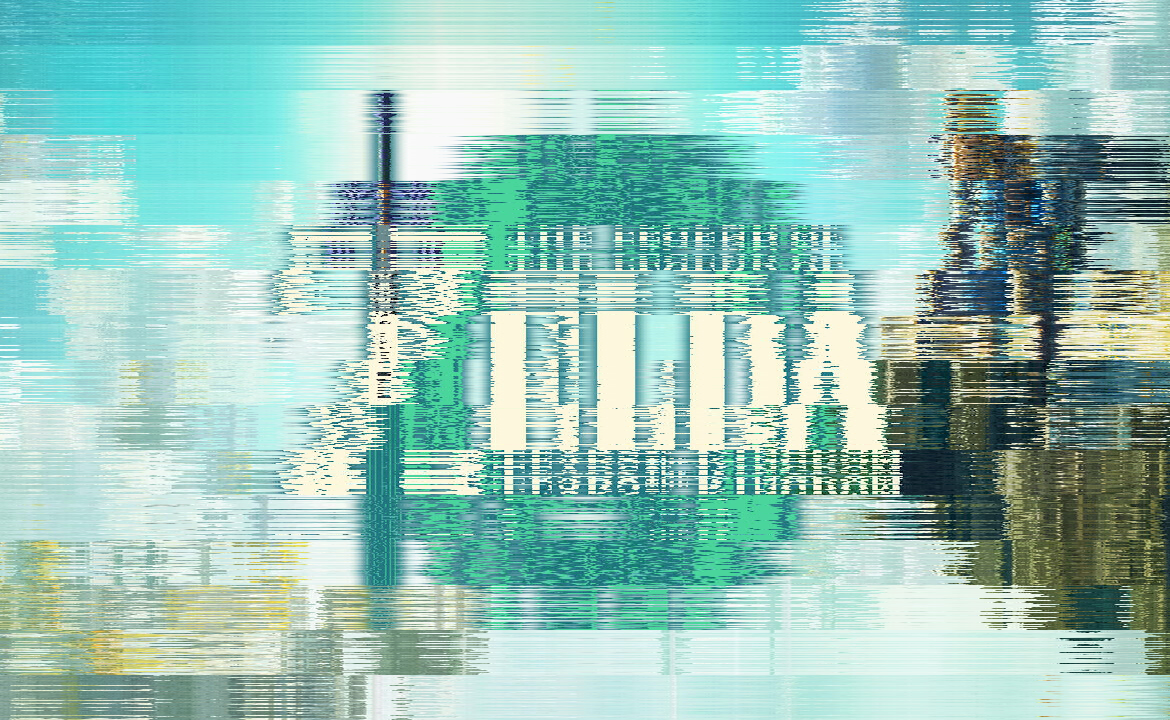
\includegraphics[width=\textwidth]{./img/cipher/16_tloztotk.png}
        \caption{16 Blöcke}
    \end{subfigure}
    \caption{Verschlüsselung des Titelbilds von The Legend Of Zelda: Tears of the Kingdom}
    \label{fig:permutation_encryption_demo}
\end{figure}
Ist die Blockanzahl gering, gibt es mehr Anordnungen der Zeilen pro Block, wodurch das Bild
undeutlicher wird (siehe Abbildung \ref{fig:permutation_encryption_demo}). Bei einer
hohen Blockanzahl wird das Bild deutlicher, da es weniger mögliche Anordnungen innerhalb eines Blocks gibt.
\subsection{Ciphtext-only Attacke}
Da ähnliche Bildzeilen oft übereinander liegen, können die sie anhand ihrer Ähnlichkeit sortiert werden. Eine Möglichkeit ist
die Zeilen Pixel für Pixel zu vergleichen und jeweils die Distanz der Farben zu berechnen. In diesem Fall sind die Pixel
im RGBA Farbraum, das bedeutet vier Bytes pro Farbkanal (Rot, Grün, Blau und Alpha). Betrachtet man die Farbkanäle als Achsen und die
Farben als Punkte in einem mehrdimensionalen Raum, kann zwischen zwei Farben einfach die euklidische Distanz berechnet werden.
\begin{figure}[h]
    \centering
    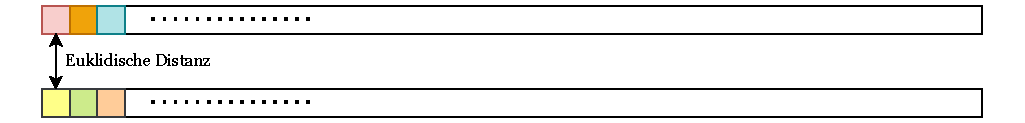
\includegraphics[width=\textwidth]{img/row_comparison.pdf}
    \caption{Zwei Bildzeilen, deren Pixel mittels euklidischer Distanz verglichen werden.}
\end{figure}
Seien $R,G,B,A\in\left[0;255\right]$ die Werte der jeweiligen Kanäle eines Pixels und $d$ die Distanz der Pixel.
\[
    d = \sqrt{(R_1 - R_2)^2 + (G_1 - G_2)^2 + (B_1 - B_2)^2 + (A_1 - A_2)^2}
\]
Die euklidische Distanz entspricht nicht umbedingt der menschlichen Wahrnehmung der Distanz zweier Farben, eignet sich allerdings
für die Sortierung der Bildzeilen. Unter den Zeilen des verschlüsselten Bilds, ist es schwierig die oberste Zeile zu identifizieren. Deshalb 
wird zur Vereinfachung angenommen, dass die oberste Zeile bereits an der richtigen Position ist. In der Realität ist das selten der Fall.
Dennoch können die Ergebnisse trotzdem erkennbar entschlüsselt werden (siehe \ref{sec:results_a15}). Von der obersten Zeile aus wird dann 
diejenige mit dem geringsten Unterschied zu den übrigen Zeilen identifiziert und mit der darauffolgenden Zeile getauscht (nearest-neighbour).

Zu Beginn werden die Zeilen des Bilds in ein Array (Vector) extrahiert, um sie später leichter zu vertauschen.
\begin{verbatim}
fn decipher(img: &RgbaImage) -> RgbaImage {
    let mut rows = img.rows()
        .map(|pixels| pixels.collect::<_>())
        .collect::<Vec<_>>();
    // ...
}
\end{verbatim}
Danach werden die Zeilen beginnend mit der obersten iteriert und der Index der besten Folgezeile bestimmt. 
Das beste Ergebnis wird dann an die nachfolgende Stelle verschoben. In diesem Fall reicht es aus, nur bis zur vorletzten Zeile
zu iterieren, da die letzte dann zwangsläufig schon die richtige Position haben muss.
\begin{verbatim}
for i in 0..img.height() as usize - 1 {
    if let Some(best_match) = nearest_neighbour(i, &rows) {
        rows.swap(i + 1, best_match);
    }
}
\end{verbatim}
Die sortierten Zeilen müssen nun nur noch zu einem neuen Bild zusammengefügt werden. Dafür wird die \verb|from_fn| Funktion der image Bibliothek verwendet,
die einfach jeden Pixel Stelle für Stelle übernimmt.
\begin{verbatim}
RgbaImage::from_fn(img.width(), img.height(), |x, y| {
    *rows[y as usize][x as usize]
})
\end{verbatim}
Die \verb|nearest_neighbour| Funktion berechnet den Index der Zeile mit der kleinsten Distanz zur Startzeile.
\begin{verbatim}
fn nearest_neighbour(start: usize, rows: &[Vec<&Rgba<u8>>]) -> Option<usize> {
    let (result, _) = (start + 1..rows.len())
        .map(|r| (r, similarity(&rows[r], &rows[start])))
        .min_by(|(_, a), (_, b)| a.partial_cmp(b).unwrap())?;
    Some(result)
}
\end{verbatim}
Die Ähnlichkeit zwischen zwei Zeilen wird anhand der euklidischen Distanz der Pixelfarben berechnet. 
Ein hoher Wert deutet auf geringe Ähnlichkeit hin, ein niedriger Wert auf hohe Ähnlichkeit.
\begin{verbatim}
fn similarity(r1: &[&Rgba<u8>], r2: &[&Rgba<u8>]) -> f32 {
    r1.iter()
        .zip(r2.iter())
        .map(|(&a, &b)| color::euclidean_distance(a.channels(), b.channels()))
        .sum()
}
\end{verbatim}
\newpage
\begin{landscape}
    \fancyhead{}
    \fancyfoot{}
    \newgeometry{left=1cm, right=-6cm, top=2.5cm, bottom=1cm}
    \renewcommand{\headrulewidth}{0pt}
\subsection{Ergebnisse}\label{sec:results_a15}
\begin{table}[h!]
    \begin{tabular}{|c|c|c|c|c|c|}
    \hline
    \textbf{Original} & \textbf{1 Block} & \textbf{4 Blöcke} & \textbf{8 Blöcke} & \textbf{16 Blöcke} & \textbf{32 Blöcke} \\
    \hline
    
\includegraphics[width=0.16\textwidth]{./img/tloztotk.png}& 
    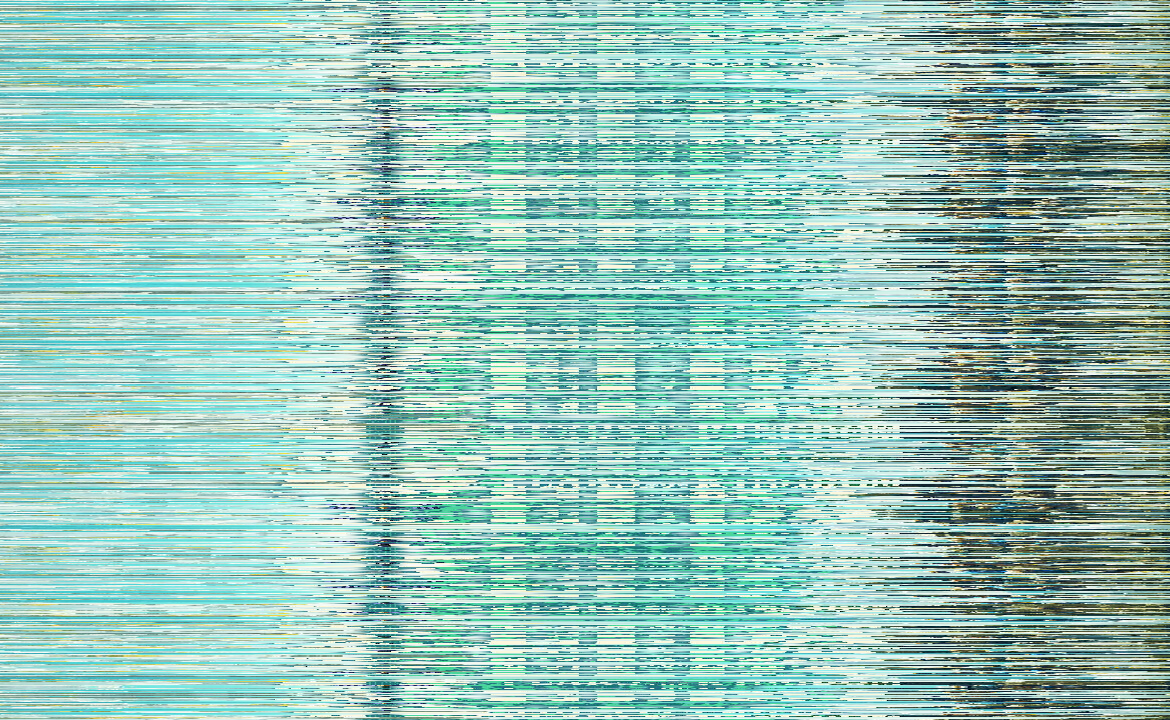
\includegraphics[width=0.16\textwidth]{./img/cipher/01_tloztotk.png}& 
    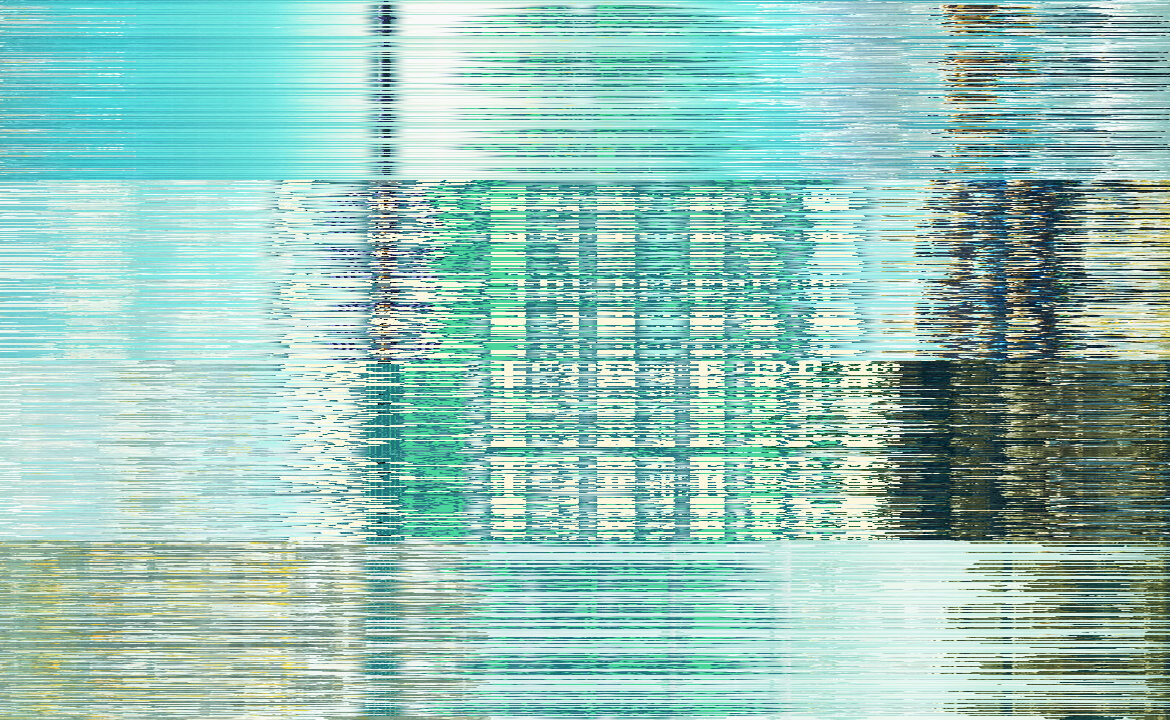
\includegraphics[width=0.16\textwidth]{./img/cipher/04_tloztotk.png}& 
    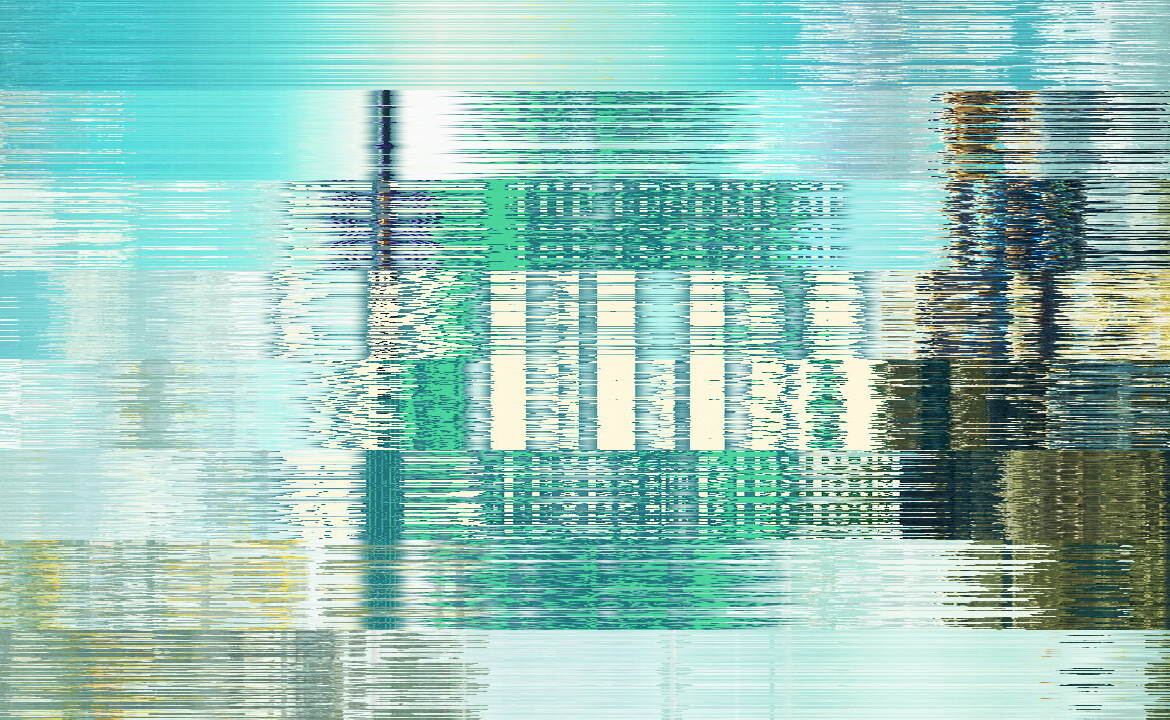
\includegraphics[width=0.16\textwidth]{./img/cipher/08_tloztotk.png}& 
    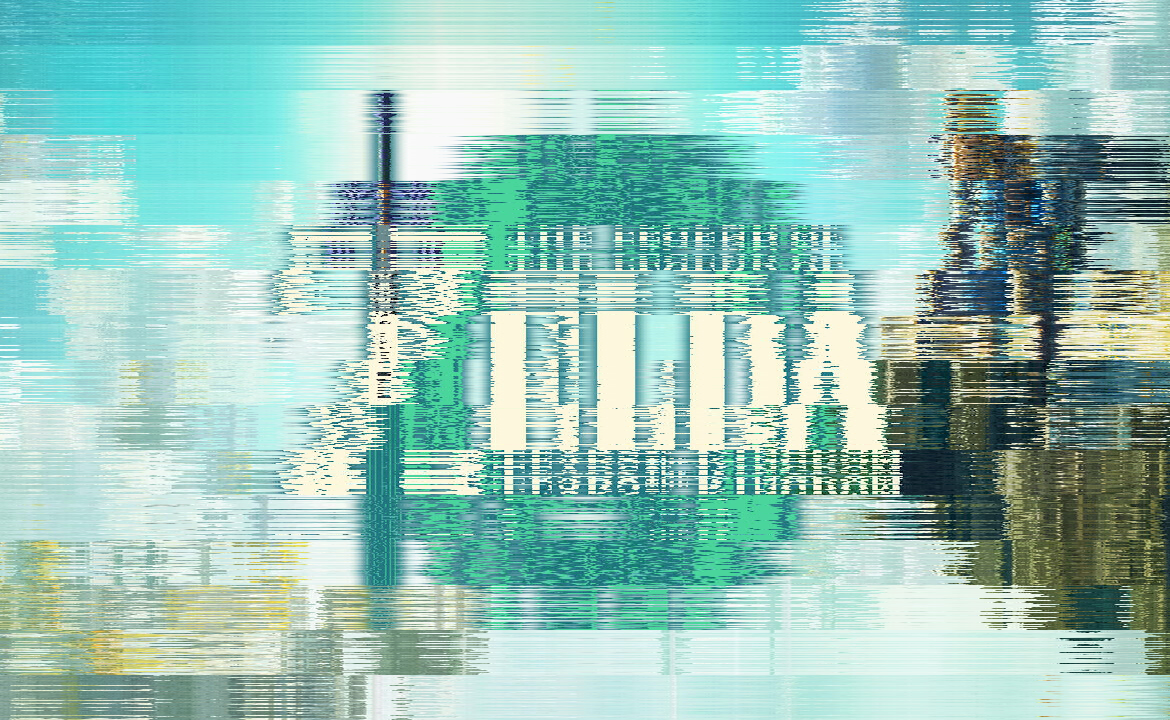
\includegraphics[width=0.16\textwidth]{./img/cipher/16_tloztotk.png}& 
    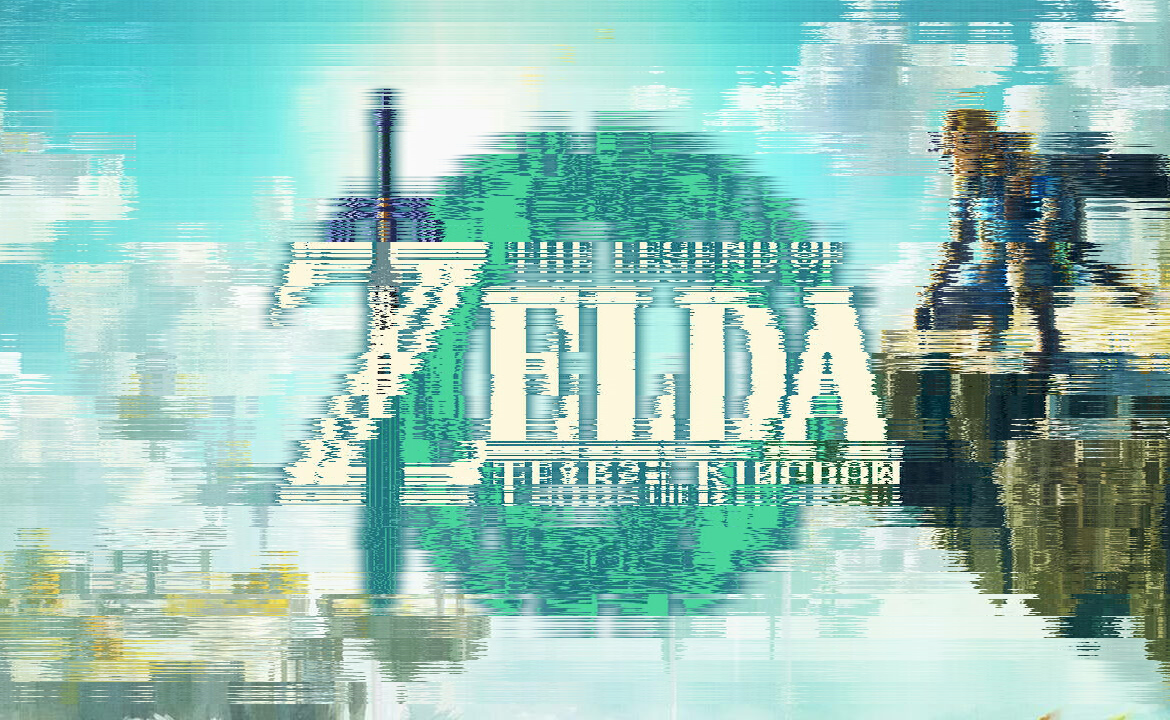
\includegraphics[width=0.16\textwidth]{./img/cipher/32_tloztotk.png}\\
    \hline
    &\textbf{Entschlüsselt 1} & \textbf{Entschlüsselt 4} & \textbf{Entschlüsselt 8} & \textbf{Entschlüsselt 16} & \textbf{Entschlüsselt 32} \\
    \hline
    &
    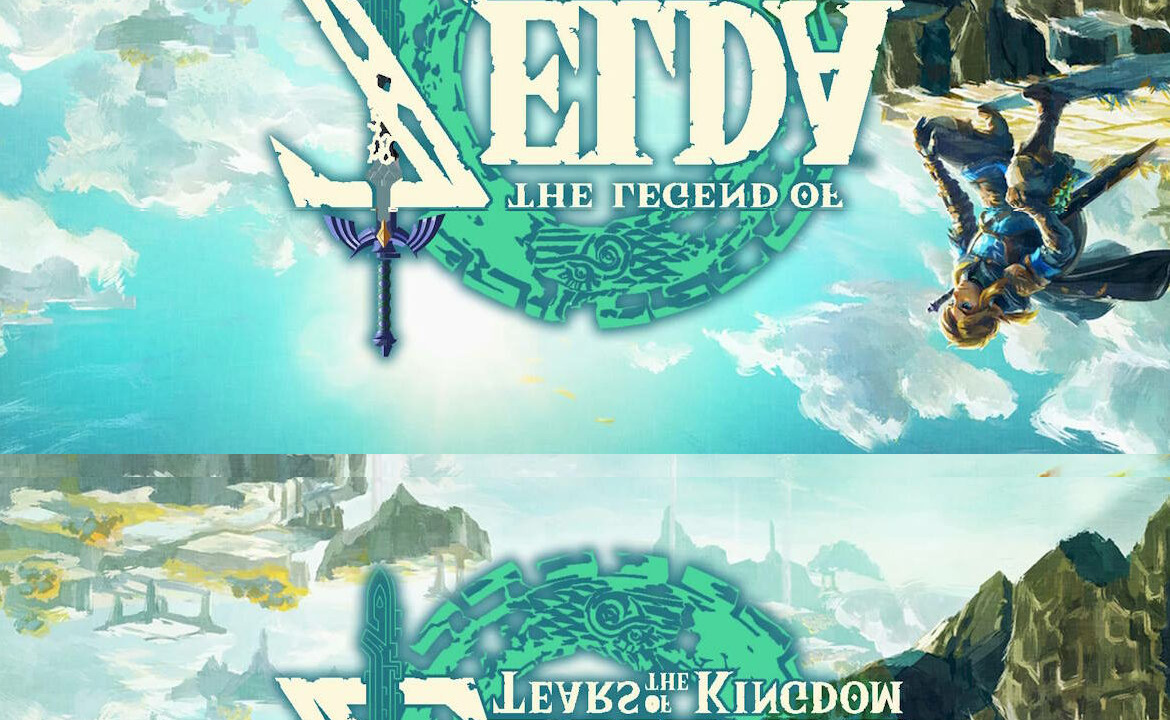
\includegraphics[width=0.16\textwidth]{./img/decipher/01_tloztotk.png}& 
    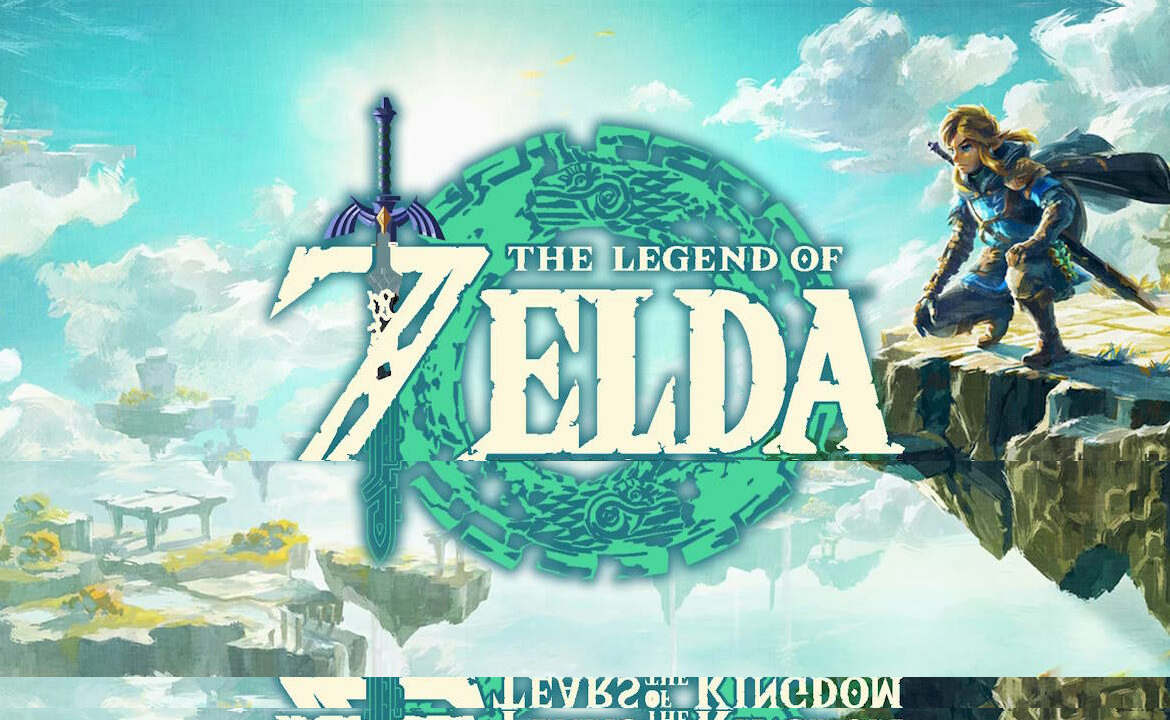
\includegraphics[width=0.16\textwidth]{./img/decipher/04_tloztotk.png}& 
    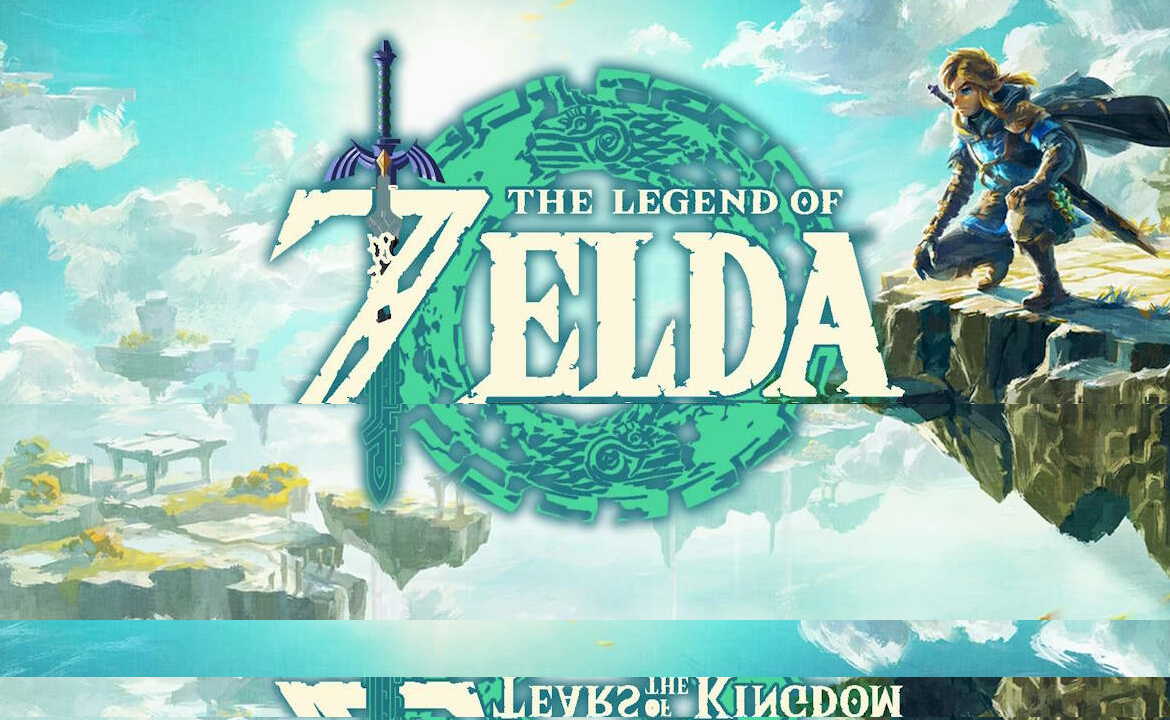
\includegraphics[width=0.16\textwidth]{./img/decipher/08_tloztotk.png}& 
    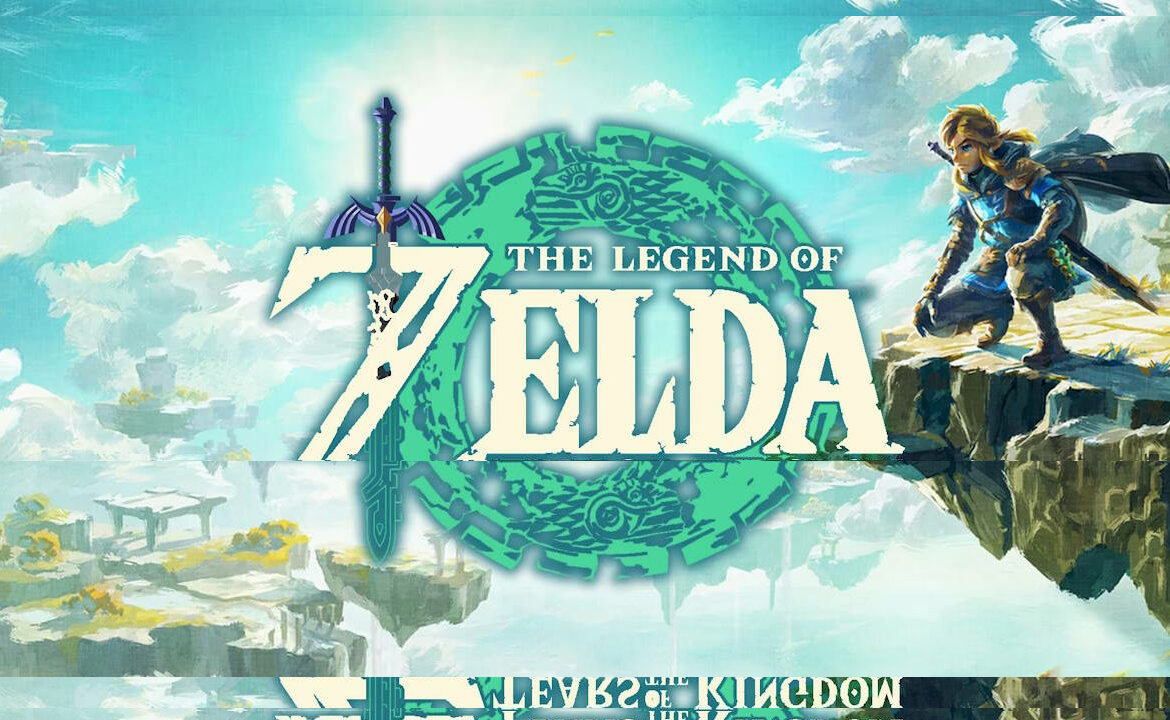
\includegraphics[width=0.16\textwidth]{./img/decipher/16_tloztotk.png}& 
    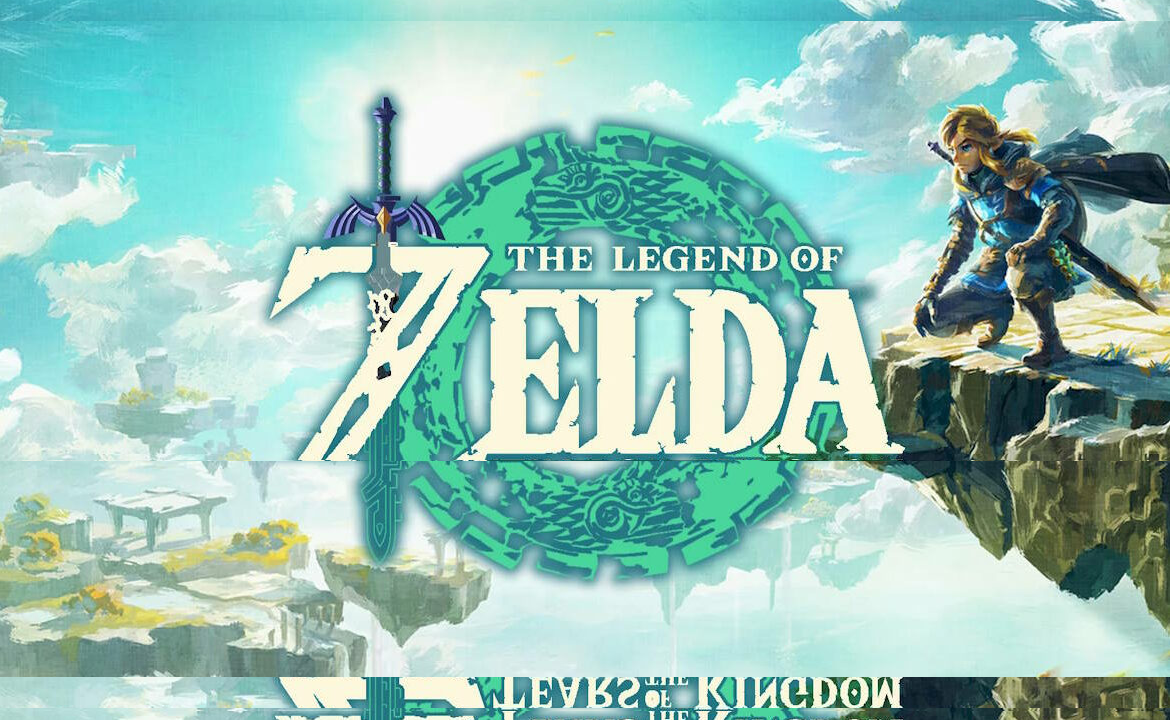
\includegraphics[width=0.16\textwidth]{./img/decipher/32_tloztotk.png}\\
    \hline
    \end{tabular}
    \caption{Originalbild Titelbild von The Legend Of Zelda: Tears of the Kingdom, verschlüsselte und entschlüsselte Versionen}
\end{table}
\begin{table}[h!]
    \begin{tabular}{|c|c|c|c|c|c|}
    \hline
    \textbf{Original} & \textbf{1 Block} & \textbf{4 Blöcke} & \textbf{8 Blöcke} & \textbf{16 Blöcke} & \textbf{32 Blöcke} \\
    \hline
    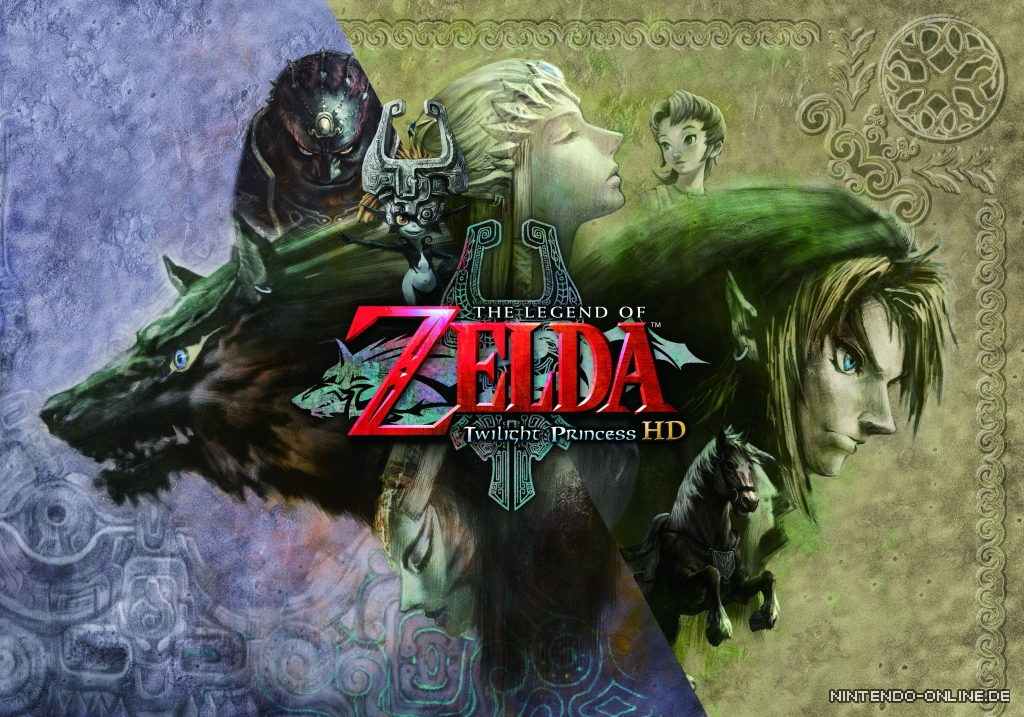
\includegraphics[width=0.16\textwidth]{./img/tloztp.png}& 
    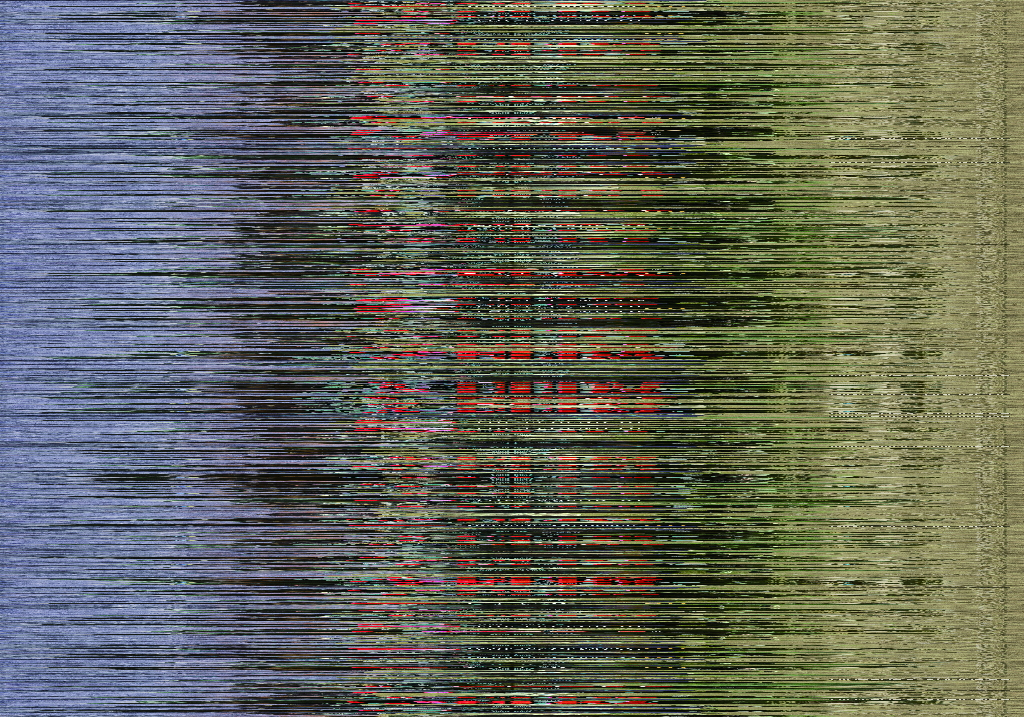
\includegraphics[width=0.16\textwidth]{./img/cipher/01_tloztp.png}& 
    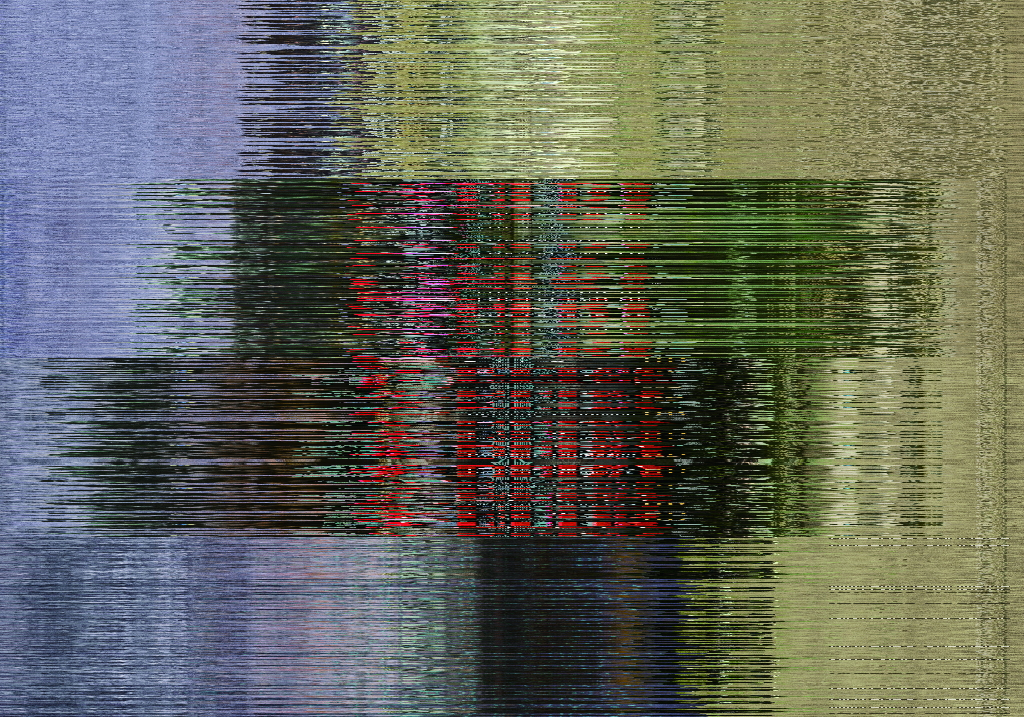
\includegraphics[width=0.16\textwidth]{./img/cipher/04_tloztp.png}& 
    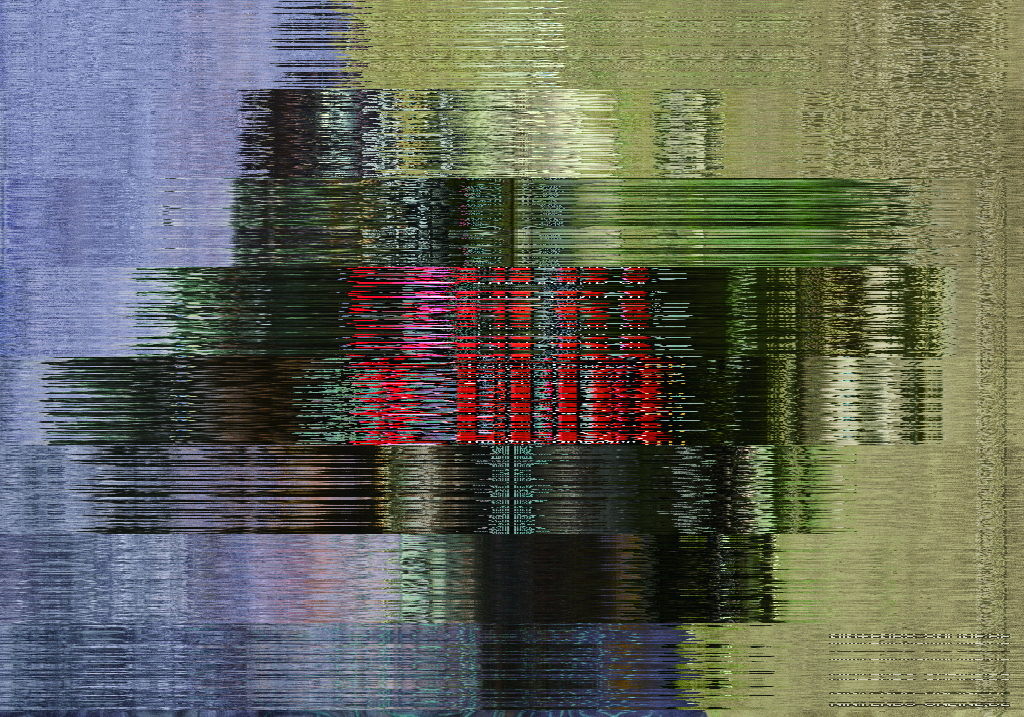
\includegraphics[width=0.16\textwidth]{./img/cipher/08_tloztp.png}& 
    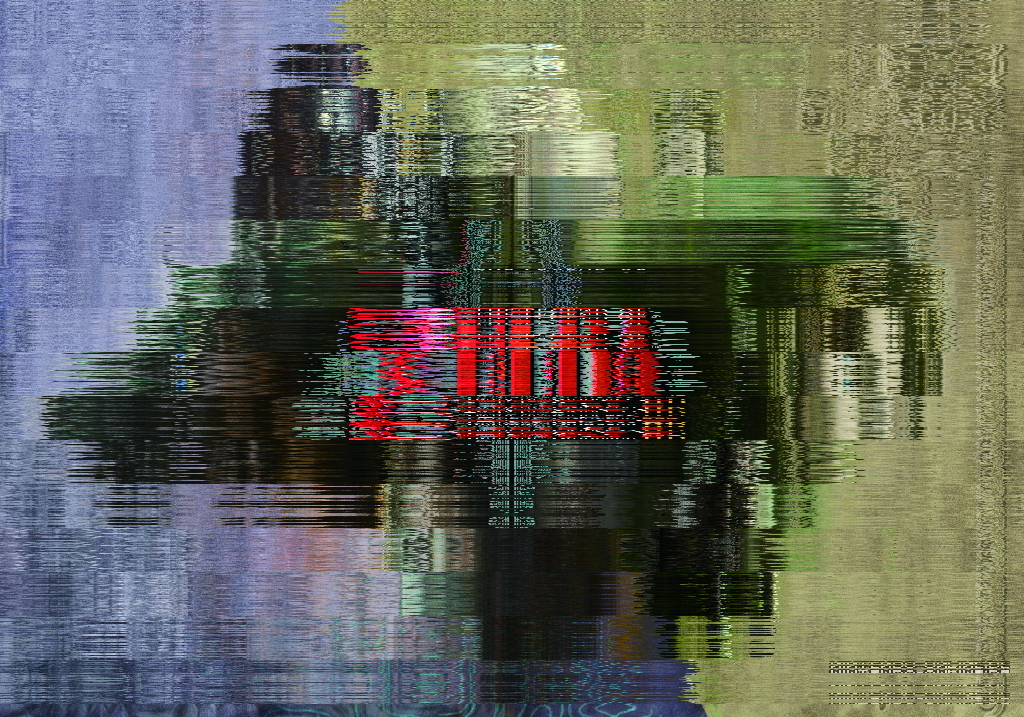
\includegraphics[width=0.16\textwidth]{./img/cipher/16_tloztp.png}& 
    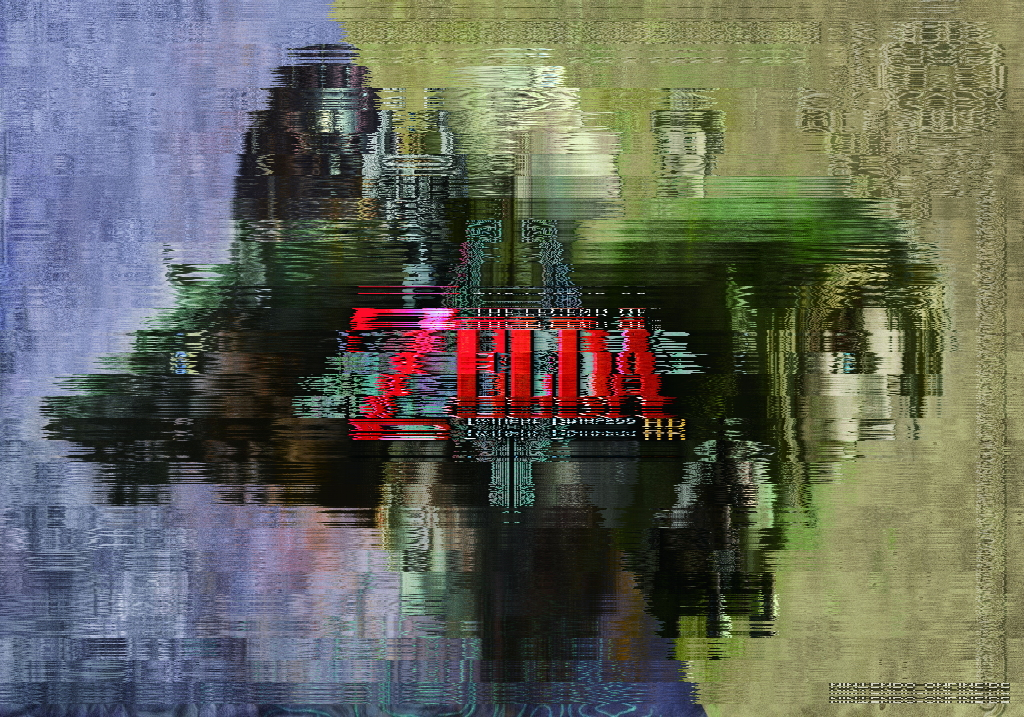
\includegraphics[width=0.16\textwidth]{./img/cipher/32_tloztp.png}\\
    \hline
    &\textbf{Entschlüsselt 1} & \textbf{Entschlüsselt 4} & \textbf{Entschlüsselt 8} & \textbf{Entschlüsselt 16} & \textbf{Entschlüsselt 32} \\
    \hline
    &
    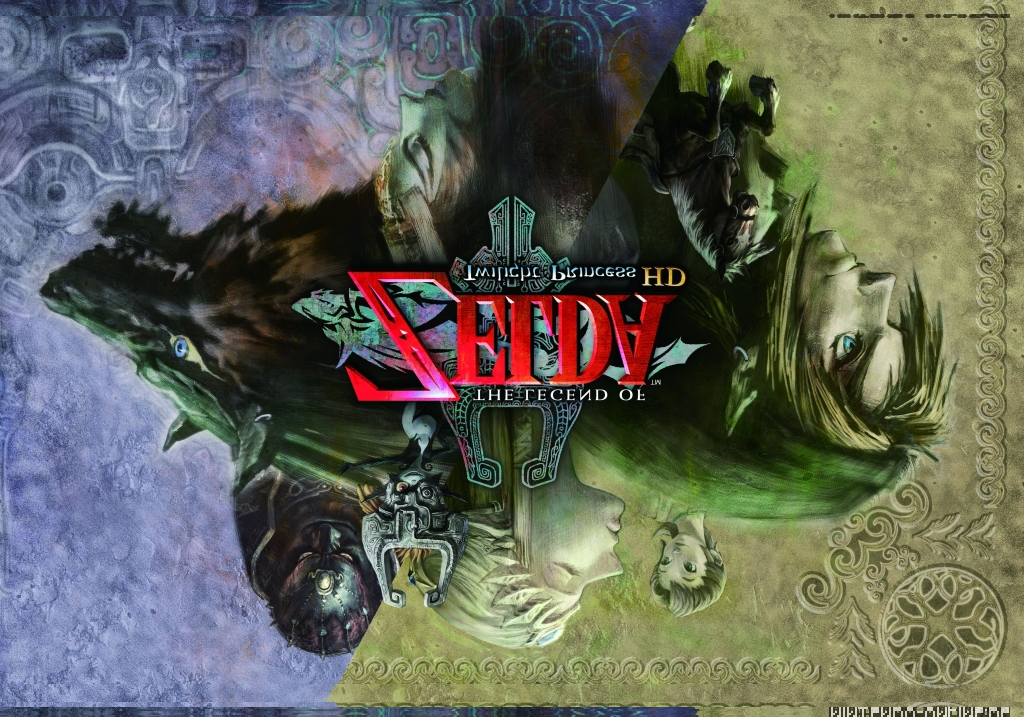
\includegraphics[width=0.16\textwidth]{./img/decipher/01_tloztp.png}& 
    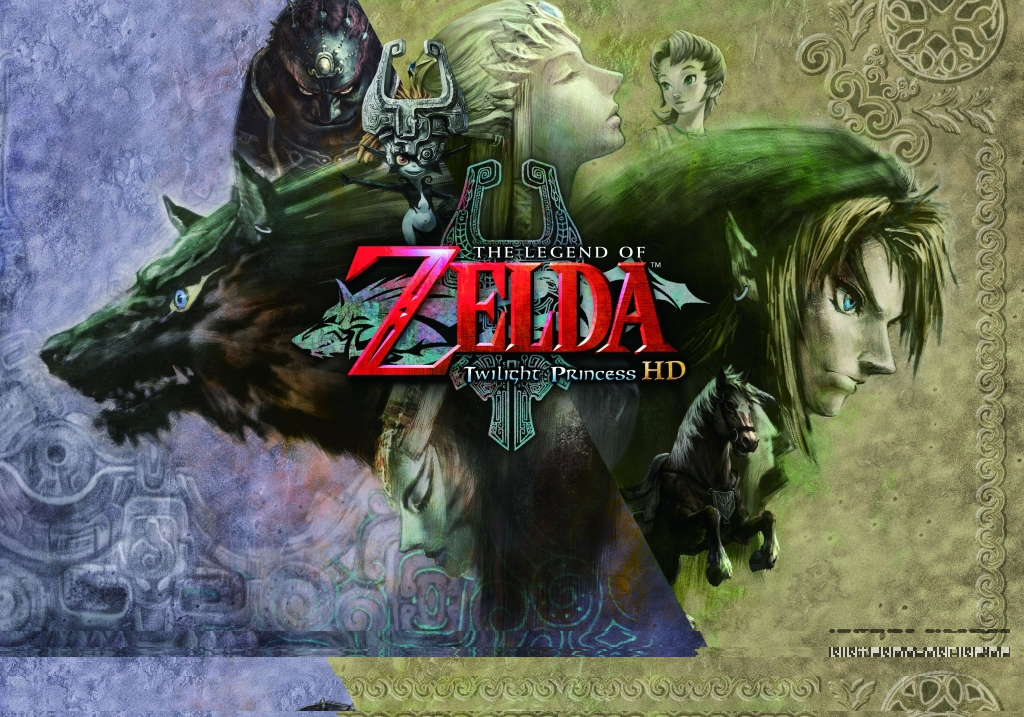
\includegraphics[width=0.16\textwidth]{./img/decipher/04_tloztp.png}& 
    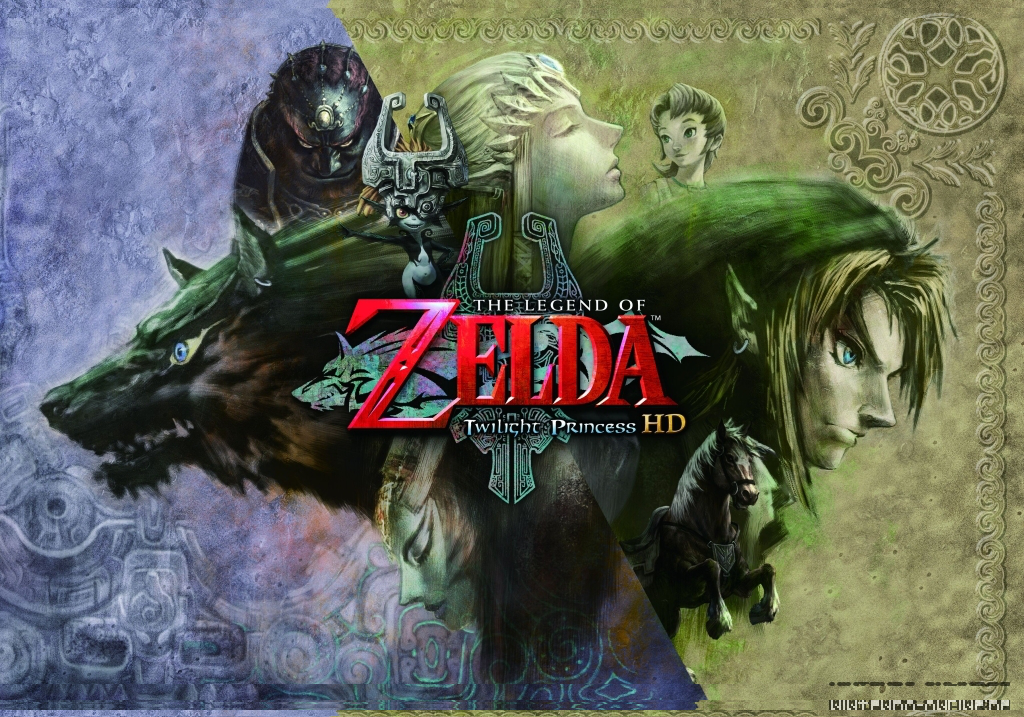
\includegraphics[width=0.16\textwidth]{./img/decipher/08_tloztp.png}& 
    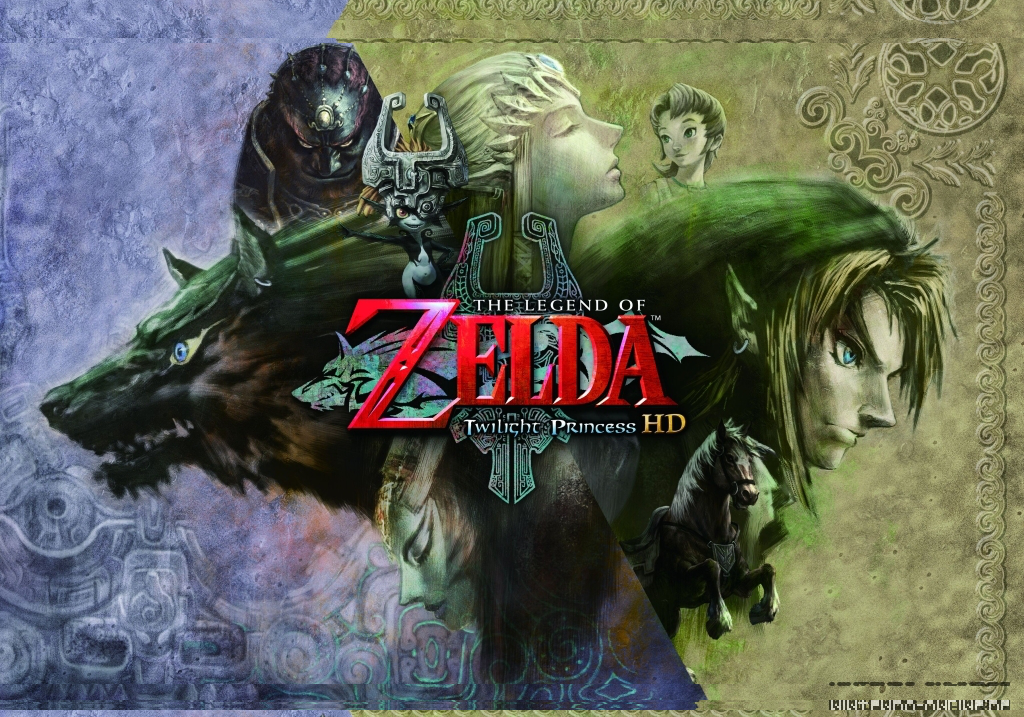
\includegraphics[width=0.16\textwidth]{./img/decipher/16_tloztp.png}& 
    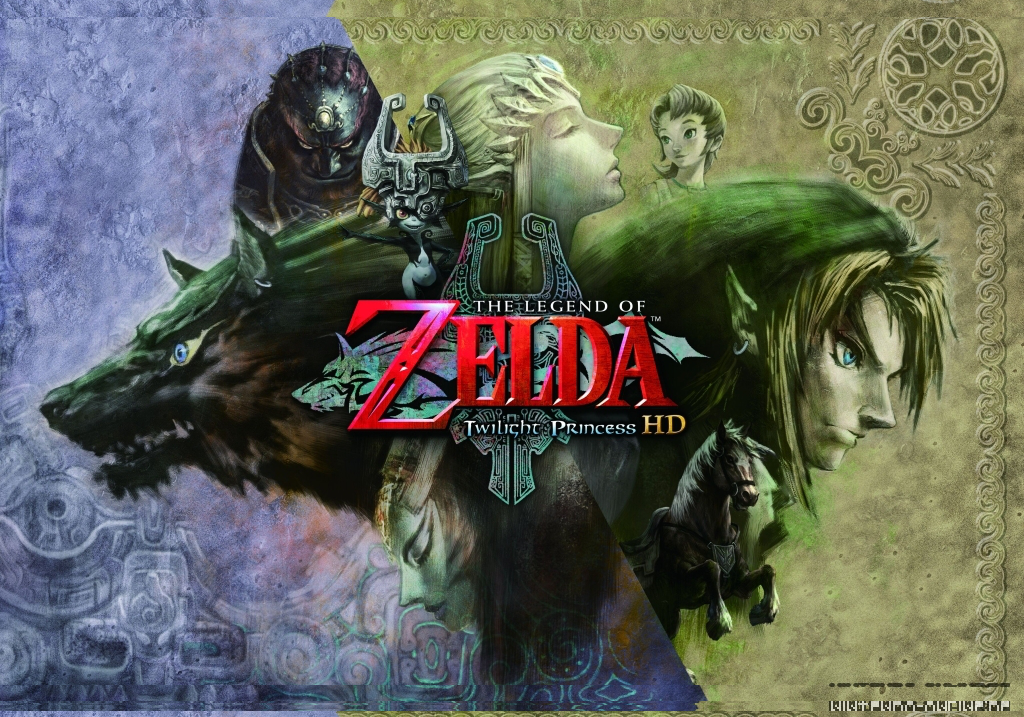
\includegraphics[width=0.16\textwidth]{./img/decipher/32_tloztp.png}\\
    \hline
    \end{tabular}
    \caption{Originalbild Titelbild von The Legend Of Zelda: Twilight Princess, verschlüsselte und entschlüsselte Versionen}
\end{table}
\newpage
\begin{table}[h!]
    \begin{tabular}{|c|c|c|c|c|c|}
    \hline
    \textbf{Original} & \textbf{1 Block} & \textbf{4 Blöcke} & \textbf{8 Blöcke} & \textbf{16 Blöcke} & \textbf{32 Blöcke} \\
    \hline
    
\includegraphics[width=0.16\textwidth]{./img/test.png}& 
    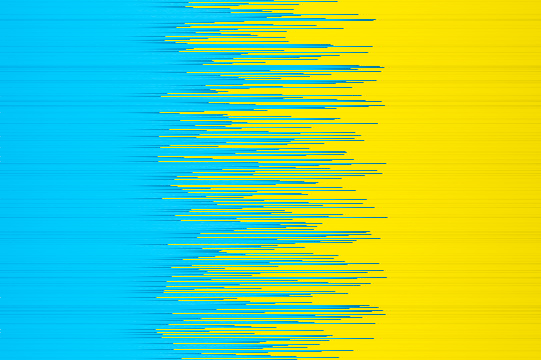
\includegraphics[width=0.16\textwidth]{./img/cipher/01_test.png}& 
    
\includegraphics[width=0.16\textwidth]{./img/cipher/04_test.png}& 
    
\includegraphics[width=0.16\textwidth]{./img/cipher/08_test.png}& 
    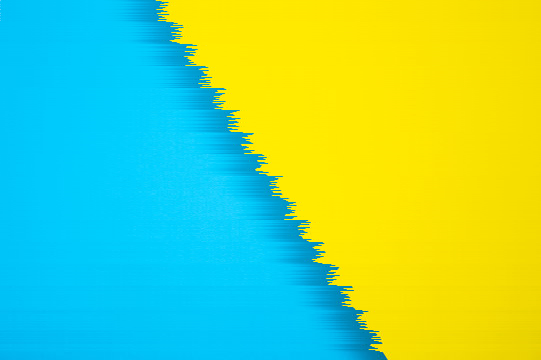
\includegraphics[width=0.16\textwidth]{./img/cipher/16_test.png}& 
    
\includegraphics[width=0.16\textwidth]{./img/cipher/32_test.png}\\
    \hline
    &\textbf{Entschlüsselt 1} & \textbf{Entschlüsselt 4} & \textbf{Entschlüsselt 8} & \textbf{Entschlüsselt 16} & \textbf{Entschlüsselt 32} \\
    \hline
    &
    
\includegraphics[width=0.16\textwidth]{./img/decipher/01_test.png}& 
    
\includegraphics[width=0.16\textwidth]{./img/decipher/04_test.png}& 
    
\includegraphics[width=0.16\textwidth]{./img/decipher/08_test.png}& 
    
\includegraphics[width=0.16\textwidth]{./img/decipher/16_test.png}& 
    
\includegraphics[width=0.16\textwidth]{./img/decipher/32_test.png}\\
    \hline
    \end{tabular}
    \caption{Zwei Farben Bild, mit schrägen Verlauf. Der Vergleich zweier Zeilen wird erleichtert.}
\end{table}
\begin{table}[h!]
    \begin{tabular}{|c|c|c|c|c|c|}
    \hline
    \textbf{Original} & \textbf{1 Block} & \textbf{4 Blöcke} & \textbf{8 Blöcke} & \textbf{16 Blöcke} & \textbf{32 Blöcke} \\
    \hline
    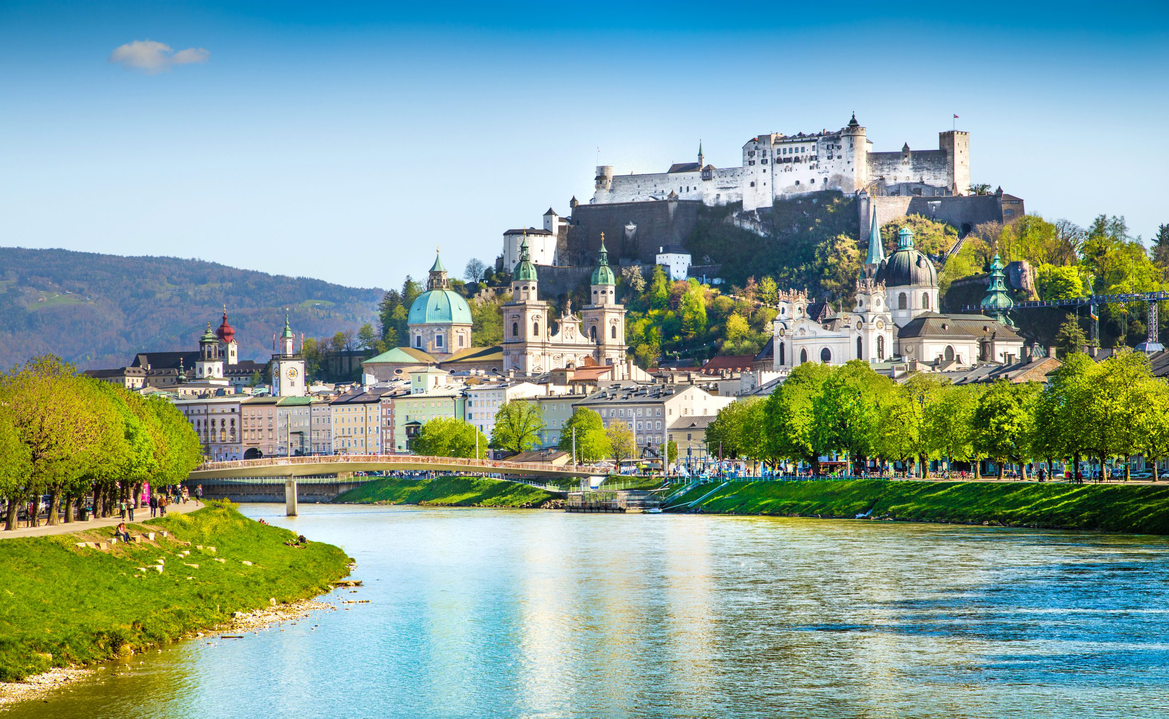
\includegraphics[width=0.16\textwidth]{./img/salzburg.png}& 
    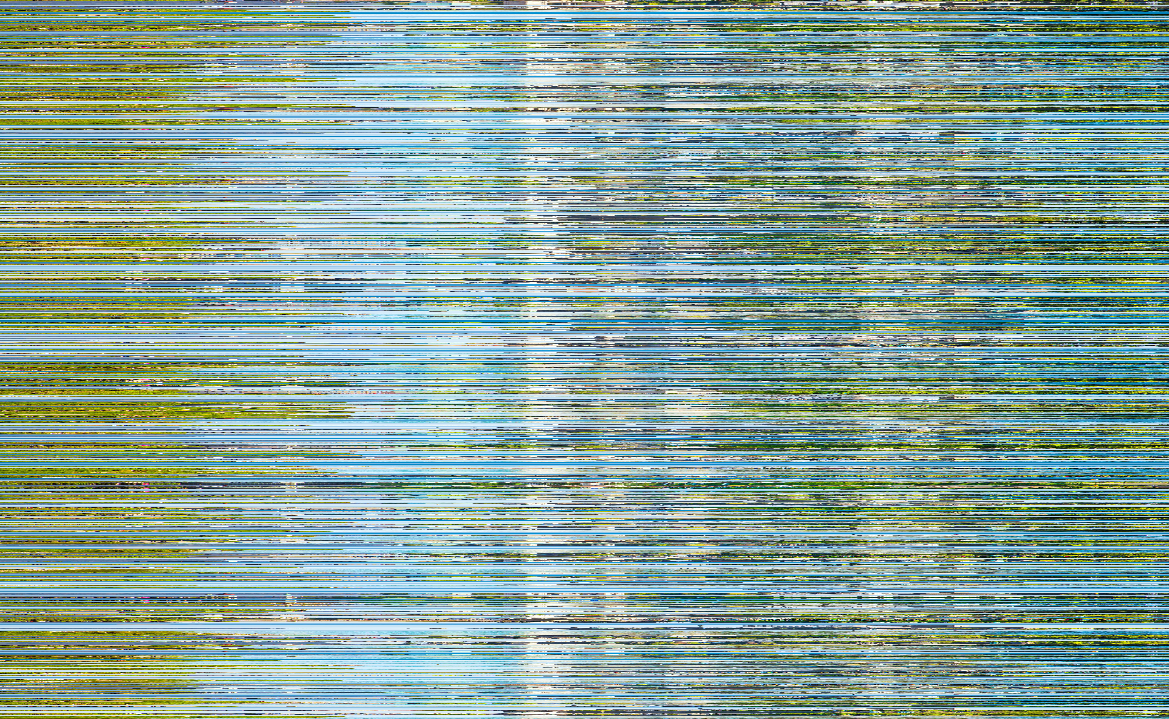
\includegraphics[width=0.16\textwidth]{./img/cipher/01_salzburg.png}& 
    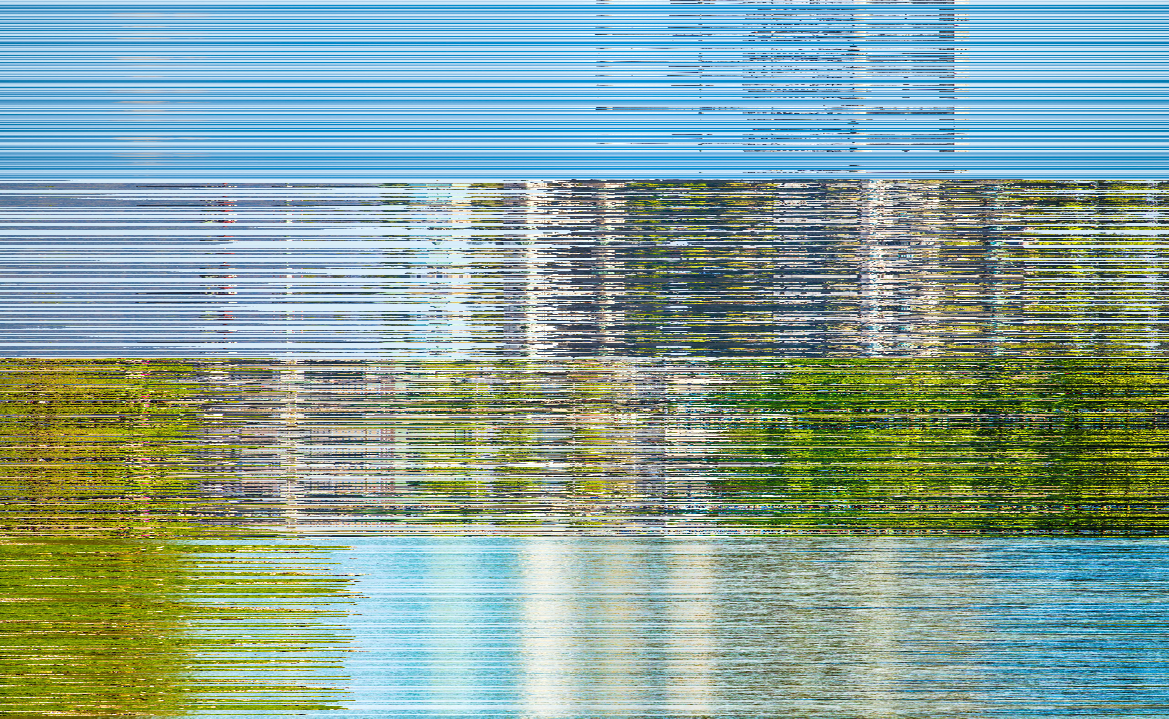
\includegraphics[width=0.16\textwidth]{./img/cipher/04_salzburg.png}& 
    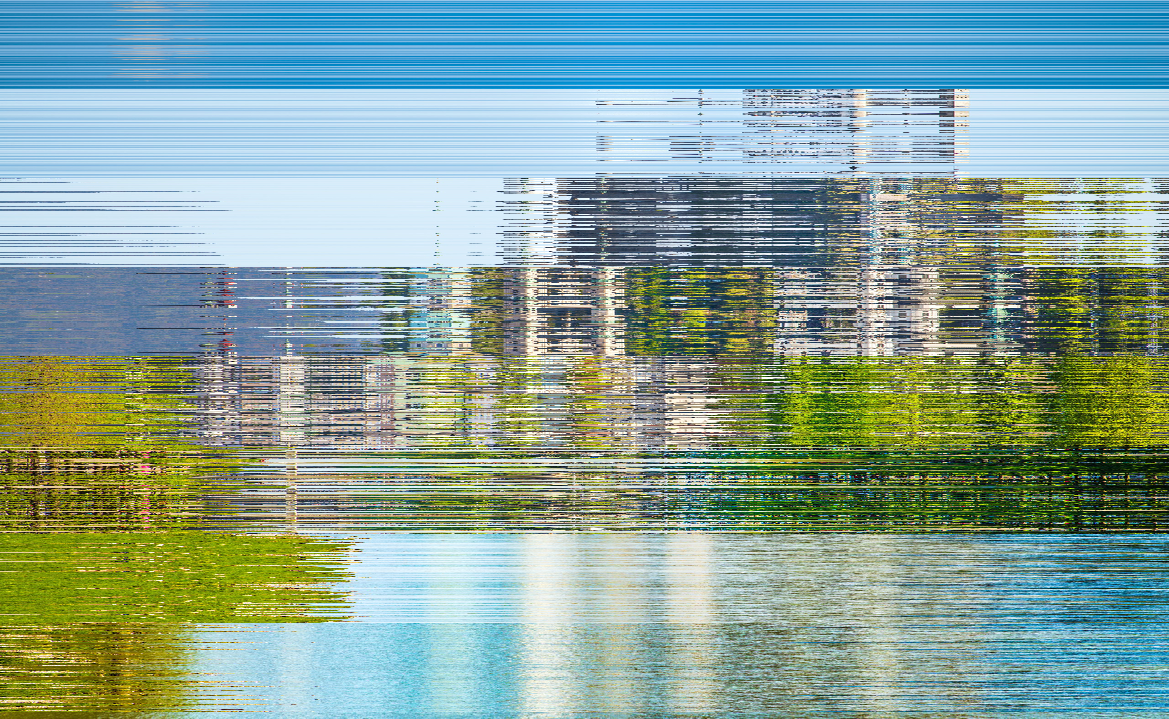
\includegraphics[width=0.16\textwidth]{./img/cipher/08_salzburg.png}& 
    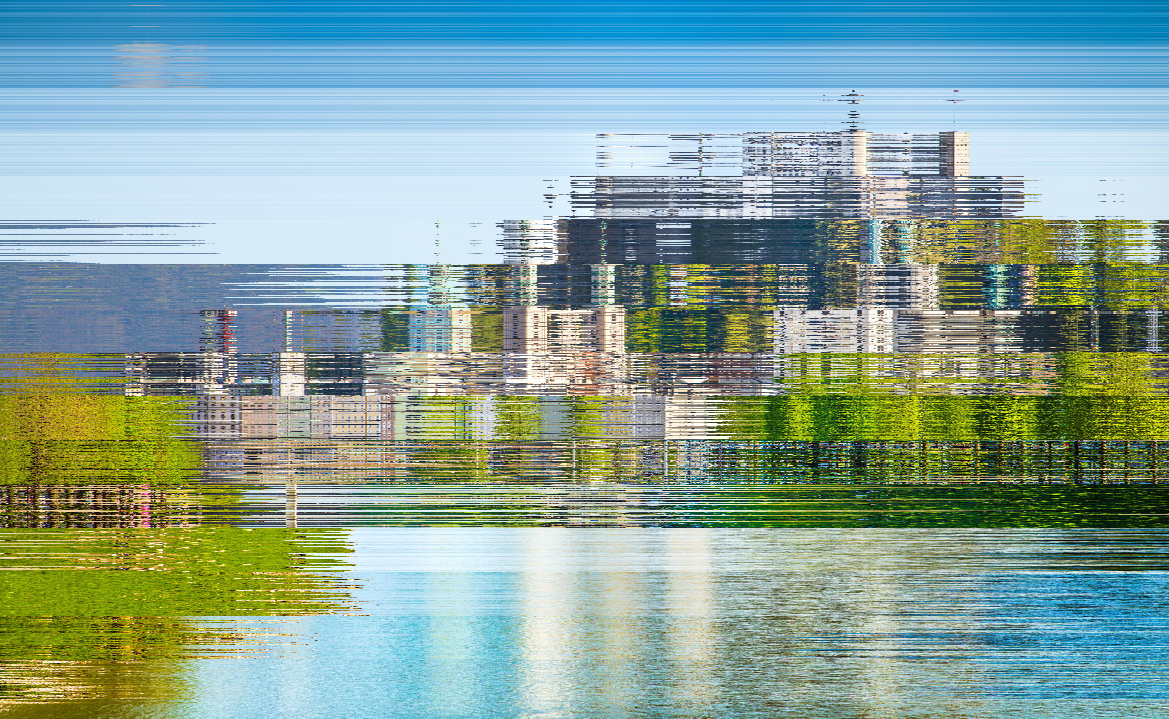
\includegraphics[width=0.16\textwidth]{./img/cipher/16_salzburg.png}& 
    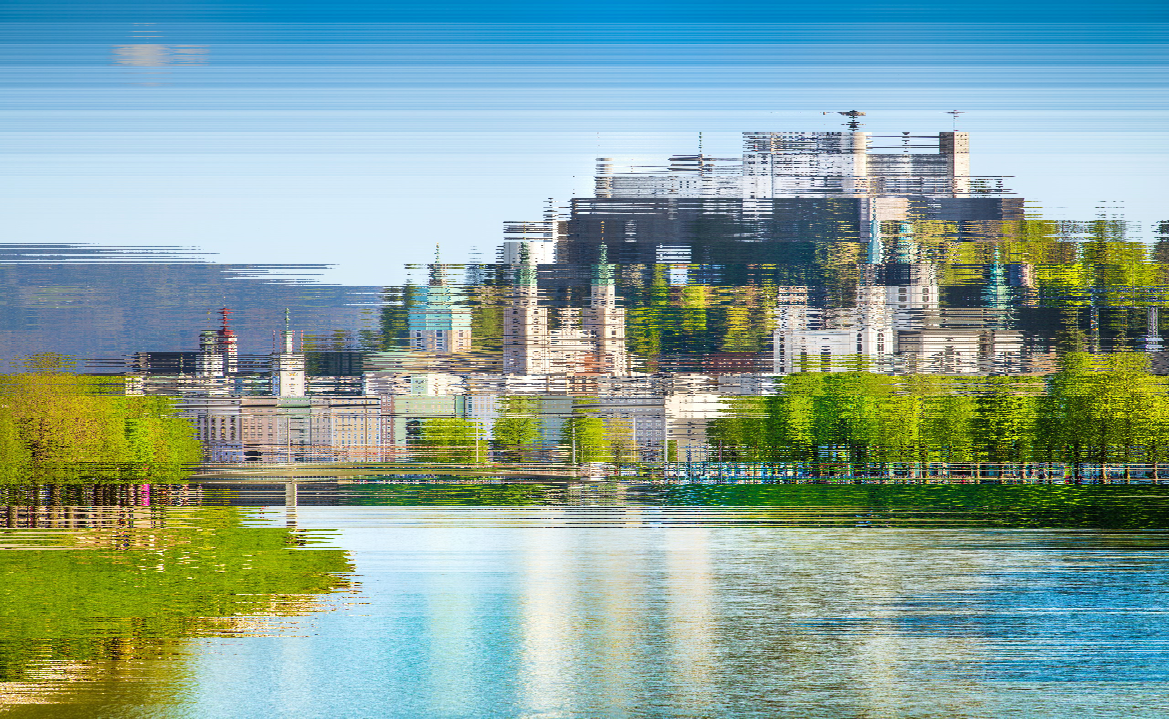
\includegraphics[width=0.16\textwidth]{./img/cipher/32_salzburg.png}\\
    \hline
    &\textbf{Entschlüsselt 1} & \textbf{Entschlüsselt 4} & \textbf{Entschlüsselt 8} & \textbf{Entschlüsselt 16} & \textbf{Entschlüsselt 32} \\
    \hline
    &
    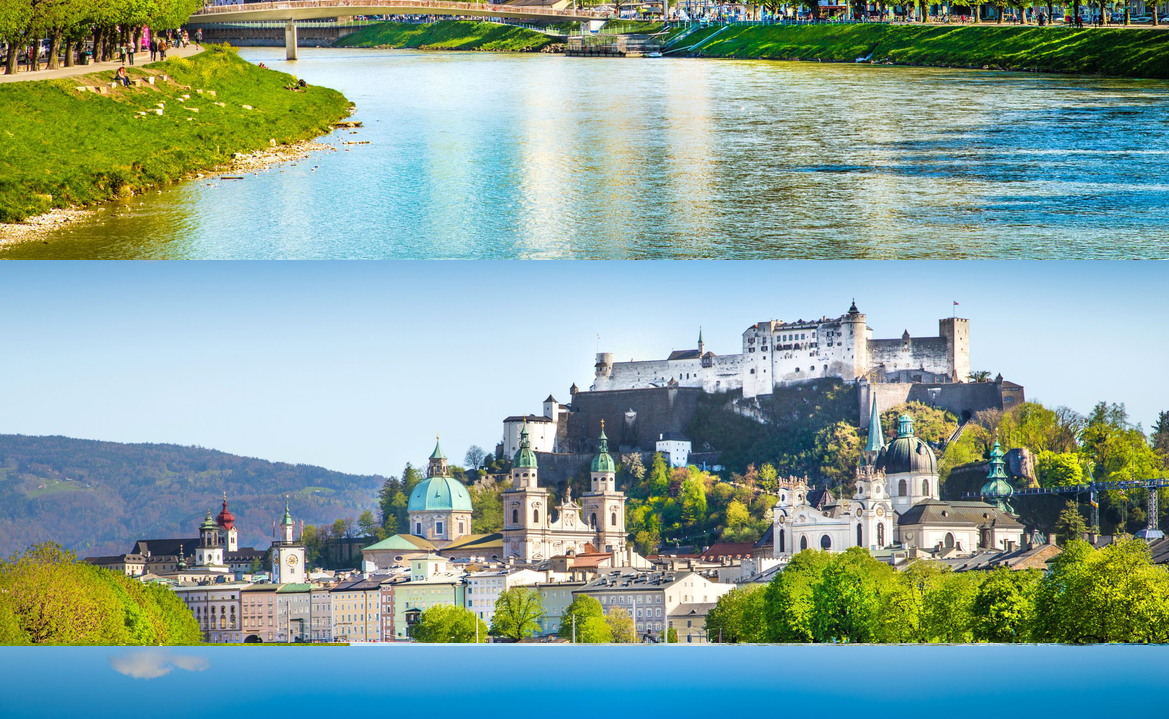
\includegraphics[width=0.16\textwidth]{./img/decipher/01_salzburg.png}& 
    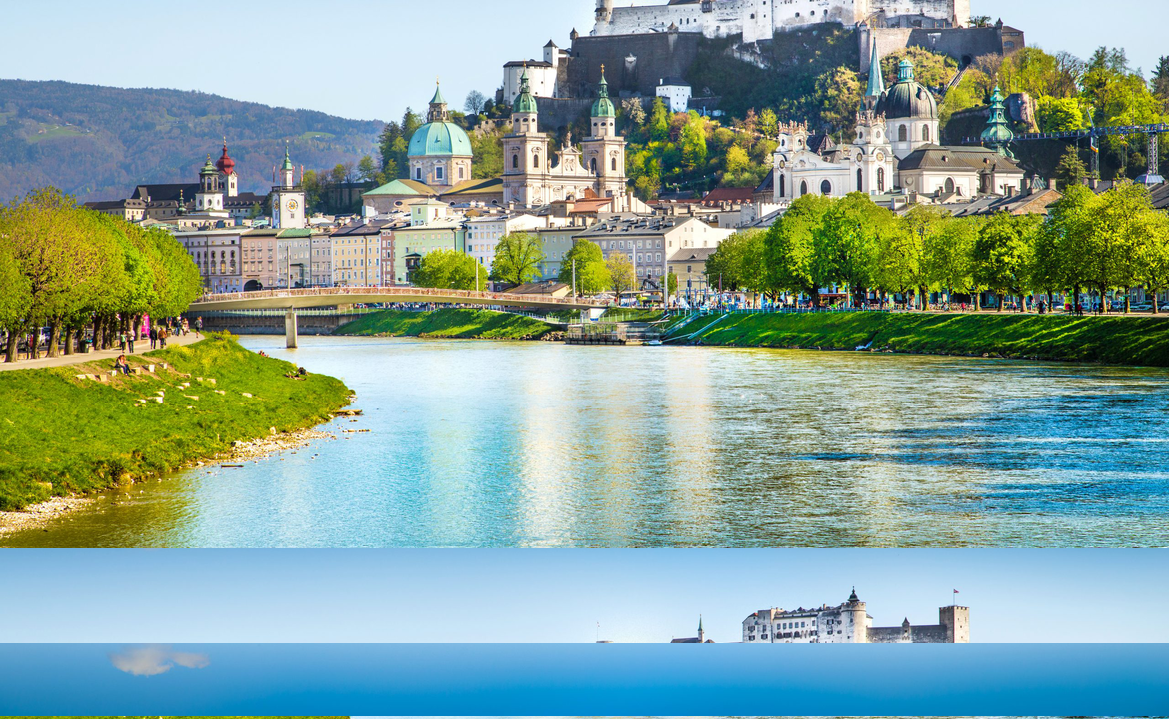
\includegraphics[width=0.16\textwidth]{./img/decipher/04_salzburg.png}& 
    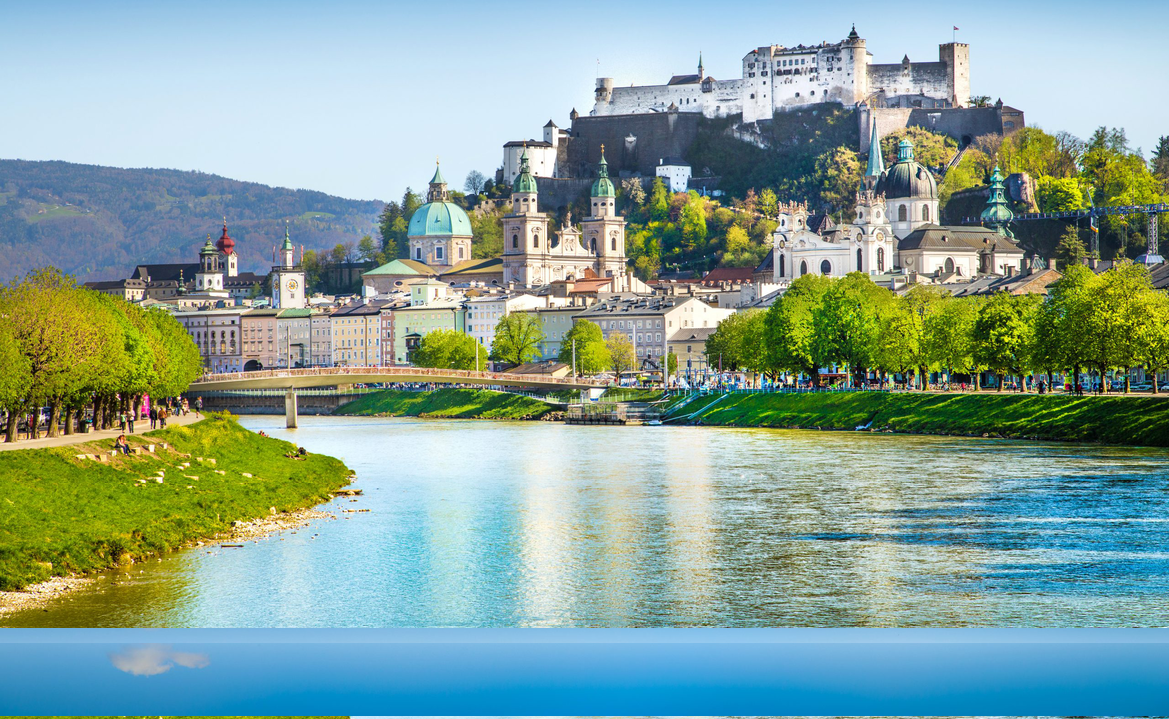
\includegraphics[width=0.16\textwidth]{./img/decipher/08_salzburg.png}& 
    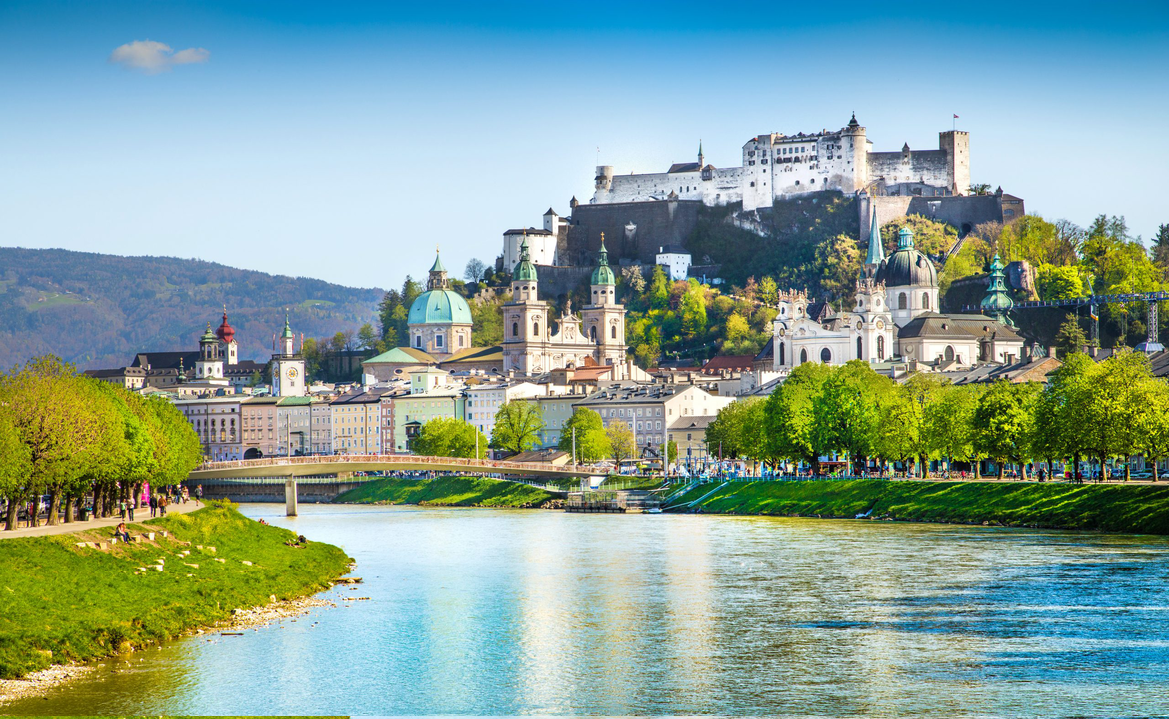
\includegraphics[width=0.16\textwidth]{./img/decipher/16_salzburg.png}& 
    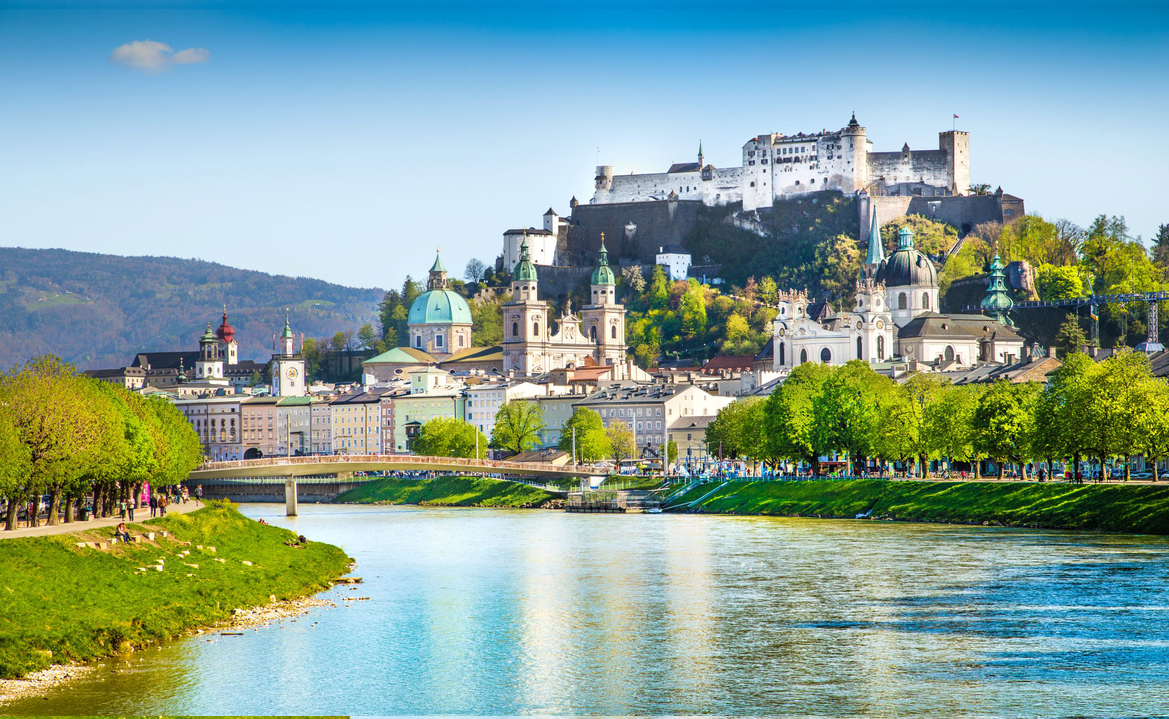
\includegraphics[width=0.16\textwidth]{./img/decipher/32_salzburg.png}\\
    \hline
    \end{tabular}
    \caption{Originalbild von Salzburg, verschlüsselte und entschlüsselte Versionen}
\end{table}
\end{landscape}
\newpage
\subsection{Fazit}
Die experimentellen Ergebnisse zeigten, dass die Blockanzahl einen entscheidenden Einfluss auf die 
Klarheit des verschlüsselten Bildes hat. Mit einer geringeren Blockanzahl wird das Bild stärker verzerrt, 
während eine höhere Blockanzahl zu einer weniger verschlüsselten Darstellung führt.
Die Ciphertext-only-Attacke, die auf der Ähnlichkeit benachbarter Bildzeilen basiert, 
konnte erfolgreich angewendet werden, wobei die Bilder Schnittstellen aufweisen oder manchmal auf dem Kopf stehen.
Die Schnittstellen sind auf die ursprüngliche Annahme, dass die erste Zeile bereits korrekt ist, zurückzuführen.
Nach der Permutation ist die oberste Zeile eine zufällige aus dem ersten Block. Je kleiner der Block ist,
desto höher ist die Wahrscheinlicht die tatsächlich richtige Zeile zu erwischen. Die darauffolgenden Zeilen
konnten richtig geordnet werden, bis eine Randzeile des Originalbilds erreicht und kein guter
Match mehr gefunden wurde. Dann wählt der Algorithmus mehr oder weniger eine zufällige der übrigen Zeilen
aus und arbeitet mit dieser weiter. Pro Zeile (exkl. Randzeilen) gibt es auch immer zwei Zeilen,
die gute Nachbarn wären. Zum einen ist das die Zeile im Originalbild, die darüber liegt und zum anderen
die darunter liegende. Je nach Wahl wird das Bild möglicherweise verkehrt herum aufgebaut.